\chapter{等質空間の幾何学}

\lectureoverview{平坦性は観測された宇宙に対する優れた近似であるが、原理ではない。等質性と等方性を保ったまま曲率を許すならば、単連結な空間幾何学としてユークリッド空間、球面空間、双曲空間の三つが現れる。それらの計量は同心の殻が距離とともにどのように成長するかから構成でき、その曲率は角度サイズと天体数によって検証できる。平坦空間も、その位相がトーラス状であれば有限でありうる。最後に、これらの等質空間のいずれかに時間依存のスケール因子を付与すれば、宇宙論的時空計量とハッブル則が得られる。そのスケール因子の力学は一般相対性理論から与えられなければならない。}

\section{平坦性は原理ではなく観測である}

これまで我々は空間を平坦として扱い、時空の幾何学についてはほとんど何も述べてこなかった。観測は平坦空間を非常に良い近似として正当化するが、平坦性を法則に高めるものではない。測定が実際に教えてくれるのは、曲率半径が我々が調査した領域に比べて大きくなければならないということである。空間は厳密に平坦かもしれないし、正の曲率をもつかもしれないし、負の曲率をもつかもしれない。観測可能な領域をはるかに超えるスケールでは、どの記述が正しいかを我々はまだ知らない。

そこで我々は一方の仮定を緩め、他方は保つ。平坦性は仮定しないが、空間が等質かつ等方であることは引き続き仮定する。これは作業仮説であり、信仰箇条ではない。その帰結を知るために、我々はそれを仮定して計算する。その後でそれを放棄し、非等質な宇宙なら何が異なるかを問うてもよい。

等質性とは、すべての点が同じ幾何学的性格をもつことを意味する。別の場所へ移動して局所的な幾何学の実験を繰り返す観測者は、同じ結果を得る。等方性とは、どの方向も特別でないことを意味する。これらの条件は、まず描かれるほとんどすべての曲面を排除する。放物面は先端付近で遠方よりも強く曲がっている。長い楕円体は極とくびれで異なる。凹凸のある球面、あるいは山や谷を分解した地球表面は、曲がっているが等質ではない。宇宙論的な問いはより狭い：
\begin{quote}
どのような空間が、すべての点から、すべての方向に、幾何学的に同じに見えながら、なお曲がりうるのか。
\end{quote}

大域的な同一視をしばらく無視すれば、定曲率の答えは三つある。平坦空間、正の曲率をもつ球面空間、負の曲率をもつ双曲空間である。大域的な同一視に関する但し書きは重要である。後に我々は平坦で有限なトーラスを構成し、これら三つで可能なすべてが尽くされるという単純化しすぎた記述を訂正する。

\section{計量と観測者の座標}

まず時空ではなく空間そのものを論じる。その幾何学は計量に符号化される。すなわち、隣接する点の間の距離の二乗\(ds^2\)を与える規則である。この局所的な規則が至る所でわかれば、長さ、角度、面積、体積、測地線、曲率はすべてそこから復元できる。

ユークリッド平面とユークリッド三次元空間に対して、デカルト座標は次を与える。
\begin{equation}
ds_2^2=dx^2+dy^2,
\qquad
ds_3^2=dx^2+dy^2+dz^2.
\label{eq:c03-cartesian-flat}
\end{equation}
第三の次元を加えることは直交する項\(dz^2\)を加えるだけであるが、重要な点はこの式の単純さではない。式~\eqref{eq:c03-cartesian-flat}が局所幾何学を完全に指定するということである。

\begin{figure}[htbp]
\centering
\includegraphics[width=0.74\textwidth]{lecture_03_figure_02.png}
\caption{黒板に書かれた平坦三次元空間のデカルト計量。}
\label{fig:c03-cartesian-board}
\lectureframe{00:05:13.138}
\end{figure}

デカルト座標は、天文学者が宇宙と出会う仕方を覆い隠す。我々は一点を占め、方向によって外を見て、見えるものを角度と距離によって分類する。二次元宇宙では、視野は文字通り我々の周りの方向の円になる。したがって極座標は単に優雅なだけでなく、宇宙論が用いる角度幾何学を明らかにする。

\(r\)を動径距離、\(\theta\)を方向とする。同じユークリッド平面は今や計量
\begin{equation}
ds^2 = dr^2 + r^2 d\theta^2.
\label{eq:c03-polar-flat}
\end{equation}
をもつ。固定された小さな角度\(d\theta\)に対して、横方向の間隔は\(r\,d\theta\)である。それは外へ向かうにつれて線形に成長し、したがって計量へのその二乗の寄与は\(r^2d\theta^2\)である。

角度の項それ自体が一次元空間の計量である。円は一次元球面であり、\(S^1\)と表記され、単位円の計量は慣例的に
\begin{equation}
d\Omega_1^2 = d\theta^2,
\qquad\text{so that}\qquad
ds^2 = dr^2 + r^2 d\Omega_1^2.
\label{eq:c03-omega-one}
\end{equation}
と書かれる。黒板には判読可能な添字のない\(d\Omega^2\)が書かれているが、口頭の定義が意図された対象を\(d\Omega_1^2\)として確定する。

\begin{figure}[htbp]
\centering
\includegraphics[width=0.74\textwidth]{lecture_03_figure_03.png}
\caption{平坦空間の極座標のスケッチと計量。黒板には\(d\Omega^2\)が示されているが、説明はそれを単位円の計量\(d\Omega_1^2=d\theta^2\)であると同定する。}
\label{fig:c03-polar-board}
\lectureframe{00:08:37.254}
\end{figure}

\begin{figure}[htbp]
\centering
\begin{tikzpicture}[scale=1.2]
\draw[->] (-1.2,0)--(1.8,0);
\draw[->] (0,-1.2)--(0,1.8);
\draw[thick] (0,0)--(1.3,1.1);
\draw (0.7,0.7) node[above] {$r$};
\draw (0.58,0) arc (0:40:0.58);
\draw (0.8,0.22) node {$\theta$};
\end{tikzpicture}
\caption{式~\eqref{eq:c03-omega-one}で用いた観測者中心の極座標を明快に再構成したものである。}
\label{fig:c03-polar-redraw}
\end{figure}

\begin{classroomqa}
\audiencequestion{\(d\theta^2\)は本当に円周に沿った距離を測るのか。}
\lecturerresponse{はい。単位円上では弧の長さはラジアン単位の角度に等しいので、\(d\theta\)だけ離れた隣接点の内在的隔たりの二乗は\(d\theta^2\)である。円の円周は\(2\pi\)であり、\(ds=d\theta\)を円周に沿って一周積分するとちょうど\(2\pi\)が得られる。\(r^2\)を掛けると単位円は平面上の半径\(r\)の殻に拡大される。\lecturetimestamp{00:09:11--00:09:26}}
\end{classroomqa}

\emph{内在的}という語が本質的である。単位円をユークリッド平面に埋め込むなら、それを次で記述できる。
\begin{equation}
x^2 + y^2 = 1.
\end{equation}
この方程式は円がより大きな空間の中にどのように位置するかを記述する。円に沿った距離しか測れない住人には必要ない。伸縮性のある光ファイバーを引き伸ばすことなく歪んだ閉ループに曲げることができる。平面上での見え方は変わるが、その内在的な円周と計量は変わらない。\(\theta\)の等しい増分は依然としてファイバーに沿った等しい距離を印す。したがって幾何学は、埋め込みがもたらす偶発的な形から切り離されねばならない。

\begin{figure}[htbp]
\centering
\includegraphics[width=0.64\textwidth]{lecture_03_figure_04.png}
\caption{黒板は丸い単位円と変形した閉ループを比較している。ループを引き伸ばさずに曲げるなら、両者は同じ内在的な一次元計量をもつ。}
\label{fig:c03-intrinsic-board}
\lectureframe{00:10:34.205}
\end{figure}

\begin{figure}[htbp]
\centering
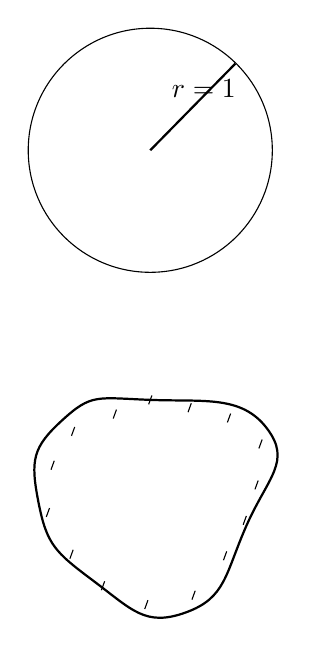
\begin{tikzpicture}[scale=1.0]
\draw (0,0) circle (1.55);
\draw[thick] (0,0)--(1.08,1.1);
\draw (0.68,0.78) node {$r=1$};

\begin{scope}[yshift=-4.35cm]
\draw[thick]
plot[smooth cycle, tension=0.95] coordinates
{(0,1.18) (1.48,0.82) (1.22,-0.42) (0.45,-1.52) (-0.72,-1.12) (-1.42,-0.12) (-1.12,0.92)};
\foreach \p in {(0,1.18),(0.5,1.08),(1.0,0.95),(1.4,0.62),(1.35,0.1),(1.2,-0.35),(0.95,-0.8),(0.55,-1.3),(-0.05,-1.42),(-0.6,-1.18),(-1.0,-0.78),(-1.3,-0.25),(-1.24,0.35),(-0.98,0.78),(-0.45,1.0)}{
\draw[rotate around={70:\p}] \p ++(-0.06,0) -- ++(0.12,0);
}
\end{scope}
\end{tikzpicture}
\caption{内在的距離は外在的変形を経ても保たれる。一次元の住人はどちらの埋め込みでも同じ円周を測る。}
\label{fig:c03-intrinsic-redraw}
\end{figure}

平坦空間は今や観測者の周りの入れ子になった円の族として読める。距離\(r\)にある殻は\(r\)だけ拡大された単位円のコピーであり、これはまさに因子\(r^2d\Omega_1^2\)が記録しているものである。

\section{正の曲率：閉じる殻}

球面は曲がっているが一様である。完全に丸い球面上のどの点も、他の点と幾何学的に区別されない。外部の三次元像に訴えることなくその計量を構成できる。単位\(2\)球面上に住む二次元の天文学者を想像し、その座標の原点を自分たちの位置に置く。

彼らの周りの小さな測地距離\(r\)にある円は小さい。\(r\)が増すにつれ円は成長し、球面の半周で最大の円周に達し、その後反対極点で潰れるまで縮む。この成長と収縮は時間ではなく\emph{距離}とともに起こる。この構成を通じて球面は静的である。

ここで\(r\)は中心からのユークリッド距離ではなく、単位球面に沿った角距離である。
\[
0 \le r \le \pi.
\]
\(r=0\)に選んだ原点があり、\(r=\pi/2\)に半周先の大円があり、\(r=\pi\)に対蹠点がある。殻の半径は今や\(\sin r\)なので、平坦な因子\(r^2\)は\(\sin^2r\)に置き換わる。
\begin{equation}
d\Omega_2^2 = dr^2 + \sin^2 r\, d\Omega_1^2
            = dr^2 + \sin^2 r\, d\theta^2.
\label{eq:c03-two-sphere}
\end{equation}
端点と中点は要求どおりに振る舞う。
\begin{equation}
\sin 0=0,
\qquad
\sin\frac{\pi}{2}=1,
\qquad
\sin\pi=0.
\end{equation}
したがって殻は大きさゼロから始まり、最大の大きさに達し、再び閉じる。

\begin{figure}[htbp]
\centering
\includegraphics[width=0.82\textwidth]{lecture_03_figure_05.png}
\caption{平坦空間の入れ子になった円から球面上の殻への移行。下の式はフレーム内で一部隠れているが、その口頭の導出は式~\eqref{eq:c03-two-sphere}における置き換え\(r^2\mapsto\sin^2r\)を与える。}
\label{fig:c03-spherical-board}
\lectureframe{00:16:11.701}
\end{figure}

\begin{figure}[htbp]
\centering
\resizebox{\linewidth}{!}{%
\begin{tikzpicture}[scale=0.92]
\begin{scope}[xshift=-4.15cm]
\draw[->] (-1.7,0)--(1.9,0);
\draw[->] (0,-1.7)--(0,1.9);
\draw (0,0) circle (0.45);
\draw (0,0) circle (0.9);
\draw (0,0) circle (1.35);
\draw[thick] (0,0)--(1.45,1.2);
\draw (0.56,0.18) arc (18:40:0.63);
\draw (0.94,0.44) node {$\theta$};
\end{scope}

\begin{scope}[xshift=4.15cm]
\draw (0,0) circle (2.0);
\fill (0,-2.0) circle (1.5pt);
\fill (2.0,0) circle (1.5pt);
\fill (0,2.0) circle (1.5pt);
\draw[thick] (0,-2.0) arc (-90:90:2.0);
\draw (0,-2.35) node {$r=0$};
\draw (2.75,0) node {$r=\pi/2$};
\draw (0,2.35) node {$r=\pi$};
\end{scope}
\end{tikzpicture}
}%
\caption{平坦な殻は永遠に成長するが、球面の殻は\(r=\pi/2\)で最大に成長し、\(r=\pi\)で閉じる。}
\label{fig:c03-shells-flat-sphere}
\end{figure}

記法\(d\Omega_2^2\)は単位\(2\)球面の計量を意味し、ちょうど\(d\Omega_1^2\)がその円形の殻の計量を意味するのと同じである。同じ再帰的構成は一次元高くても働く。平坦な三次元空間内の固定された半径では、我々の周りの殻は\(2\)球面である。
\begin{equation}
ds_{\text{flat},3}^2 = dr^2 + r^2 d\Omega_2^2.
\label{eq:c03-flat-three-polar}
\end{equation}
もしそれらの\(2\)球面の殻が因子\(\sin r\)とともに成長してから閉じるなら、結果として得られる空間は単位\(3\)球面である。
\begin{equation}
d\Omega_3^2 = dr^2 + \sin^2 r\, d\Omega_2^2.
\label{eq:c03-three-sphere}
\end{equation}
\(3\)球面は、その馴染みの埋め込みが四次元ユークリッド空間を必要とするため描きにくい。しかし計量は完全であり、像を必要としない。任意に選んだ観測者の周りには入れ子になった\(2\)球面が位置し、それらは最大まで成長してから反対極点まで縮む。

\begin{classroomqa}
\audiencequestion{観測者は球の中心にいるのか。}
\lecturerresponse{観測者は\emph{座標殻}の中心にいるのであって、特権的な幾何学的中心にいるのではない。原点は空間上の一点であり、他のどの観測者も自分の点を\(r=0\)として選び、同じ計量を得ることができる。一様性とは、まさにそのような選択がどれも優先されないという主張である。\lecturetimestamp{00:19:21--00:20:27}}
\end{classroomqa}

可視化のためだけに、単位円と単位\(2\)球面をユークリッド空間に埋め込むことができる。
\begin{equation}
x^2+y^2=1,
\qquad
x^2+y^2+z^2=1.
\end{equation}
これらの式は埋め込みを記述するものであり、余分な物理ではない。円や球面上に閉じ込められた蟻は、周囲のユークリッド空間を検出することなく内在的計量を決定できる。同様に、\(S^3\)は神秘的な境界をもつ通常の球ではない。それは式~\eqref{eq:c03-three-sphere}で記述される完全な三次元空間である。

\section{曲率は我々の見え方をどう変えるか}

幾何学が物理になるのは、それが観測を変えるときだけである。物体の横断直径\(d\)が既知であり、その動径距離\(r\)が独立に推定されており、その角直径\(d\theta\)が空で測定されるとしよう。銀河は粗い直観的な例を与える。より精密な宇宙論では較正された標準尺と標準光源を用いる。距離の情報は、分光赤方偏移、ハッブル関係、光度、および異なるクラスの天体間の相互較正から組み立てることができる。

平坦空間では、物体の横断幅にわたって\(r\)を固定する。式~\eqref{eq:c03-polar-flat}より
\begin{equation}
d^2 = r^2 d\theta^2.
\label{eq:c03-flat-angle-step}
\end{equation}
したがって
\begin{equation}
d\theta = \frac{d}{r}.
\label{eq:c03-flat-angle}
\end{equation}
角径は距離に反比例して小さくなる。

単位球面上では、横断殻の大きさは\(r\)ではなく\(\sin r\)である。
\begin{equation}
d^2 = \sin^2 r\, d\theta^2,
\qquad\text{hence}\qquad
d\theta = \frac{d}{\sin r}.
\label{eq:c03-spherical-angle}
\end{equation}
\(0<r<\pi\)に対して\(\sin r<r\)であるから、同じ動径距離にある同じ物体は平坦空間におけるよりも大きく見える。その角径はまず減少し、赤道で最小に達し、その後殻が収縮するにつれて増大する。対蹠点における極限的な理想化では、すべての方向が出会い、像は空全体に広がる。

\begin{classroomqa}
\audiencequestion{これは宇宙マイクロ波背景放射から曲率を推測するのと同じ考え方か。}
\lecturerresponse{はい。初期プラズマはその音響振動を通じて特徴的な物理的スケールを与える。我々はその標準尺が張る角度を測定し、各幾何学が予測する角度と比較する。物体は文字通り銀河である必要はない。本質的な比較は、既知の横断スケールとその観測された角径との対比である。\lecturetimestamp{00:37:37--00:38:12}}
\end{classroomqa}

殻の体積は第二の検証を与える。三次元平坦空間では、殻の面積は\(r^2\)に比例し、単位\(3\)球面上では\(\sin^2r\)に比例する。したがって一様な母集団は、球面殻上ではまず距離とともに数が増え、赤道を過ぎると減る。正の曲率は平坦空間に対する対をなす特徴を予測する。すなわち、十分遠方の標準尺は大きすぎるように見え、十分遠方の殻は含む天体が少なすぎる。

\begin{figure}[htbp]
\centering
\resizebox{\linewidth}{!}{%
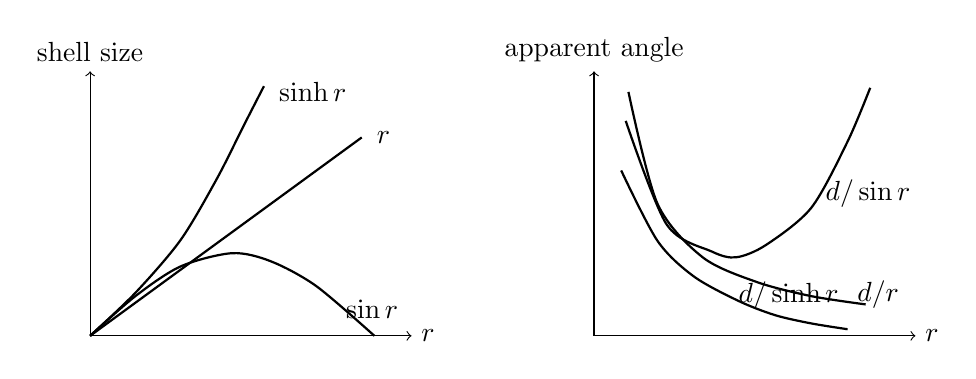
\begin{tikzpicture}[x=1.15cm,y=1.05cm]
\begin{scope}
\draw[->] (0,0)--(3.55,0) node[right] {$r$};
\draw[->] (0,0)--(0,3.2) node[above] {shell size};

\draw[thick] (0,0)--(3.0,2.4);
\draw (3.06,2.4) node[right] {$r$};

\draw[thick]
plot[smooth] coordinates {(0,0) (0.5,0.48) (1.0,0.84) (1.57,1.0) (2.0,0.9) (2.5,0.6) (3.14,0)};
\draw (2.72,0.55) node[below right] {$\sin r$};

\draw[thick]
plot[smooth] coordinates {(0,0) (0.5,0.52) (1.0,1.16) (1.4,1.9) (1.7,2.55) (1.92,3.02)};
\draw (1.98,2.95) node[right] {$\sinh r$};
\end{scope}

\begin{scope}[xshift=6.4cm]
\draw[->] (0,0)--(3.55,0) node[right] {$r$};
\draw[->] (0,0)--(0,3.2) node[above] {apparent angle};

\draw[thick]
plot[smooth] coordinates {(0.38,2.95) (0.7,1.6) (1.2,0.95) (1.8,0.65) (2.4,0.48) (3.0,0.38)};
\draw (2.8,0.5) node[right] {$d/r$};

\draw[thick]
plot[smooth] coordinates {(0.35,2.6) (0.8,1.35) (1.3,1.02) (1.57,0.95) (1.9,1.1) (2.4,1.55) (2.8,2.35) (3.05,3.0)};
\draw (2.45,1.72) node[right] {$d/\sin r$};

\draw[thick]
plot[smooth] coordinates {(0.3,2.0) (0.7,1.15) (1.1,0.72) (1.6,0.42) (2.0,0.25) (2.4,0.15) (2.8,0.08)};
\draw (2.15,0.2) node[above] {$d/\sinh r$};
\end{scope}
\end{tikzpicture}
}%
\caption{動径方向の殻の因子と対応する角径の法則。正の曲率は殻を閉じさせ、負の曲率はそれを指数関数的に成長させる。}
\label{fig:c03-shell-angular-laws}
\end{figure}

\begin{classroomqa}
\audiencequestion{球面を回り続けると動径座標は無限大になるのか。}
\lecturerresponse{いいえ。単位球面上では、\(r\)は測地線的な角距離であり、\(0\)から\(\pi\)までの範囲しかとらない。\(r=\pi\)では殻は対蹠点で潰れている。ここでは固定された空間幾何学を調べているのであって、時間とともに物体を外へ追っているのではない。後に曲率半径を導入すると、すべての物理的距離はその半径で掛けられるが、この無次元の範囲は変わらない。\lecturetimestamp{00:39:30--00:40:35}}
\end{classroomqa}

\section{射影は幾何学ではない}

負の曲率に移る前に、忠実な幾何学が絵によっていかにひどく歪められうるかを見ておくと有用である。球面をその南極で接する平面の上に置く。北極から球面上の各点\(P\)を通る直線を引き、平面との交点\(P'\)まで延ばす。これがステレオ投影である。北極自身は無限遠へ送られる。南極付近の小さな領域はほとんど歪みなく表されるが、北極付近の等しい内在的領域は平面上で巨大になる。

歪みは地図に属するものであり、球面に属するものではない。元の球面は、その平面像が等価な領域に極端に異なる座標サイズを割り当てるにもかかわらず、一様なままである。この規律は、無限の双曲空間を有限の円板に圧縮するときにも再び必要となる。

\begin{figure}[htbp]
\centering
\resizebox{\linewidth}{!}{%
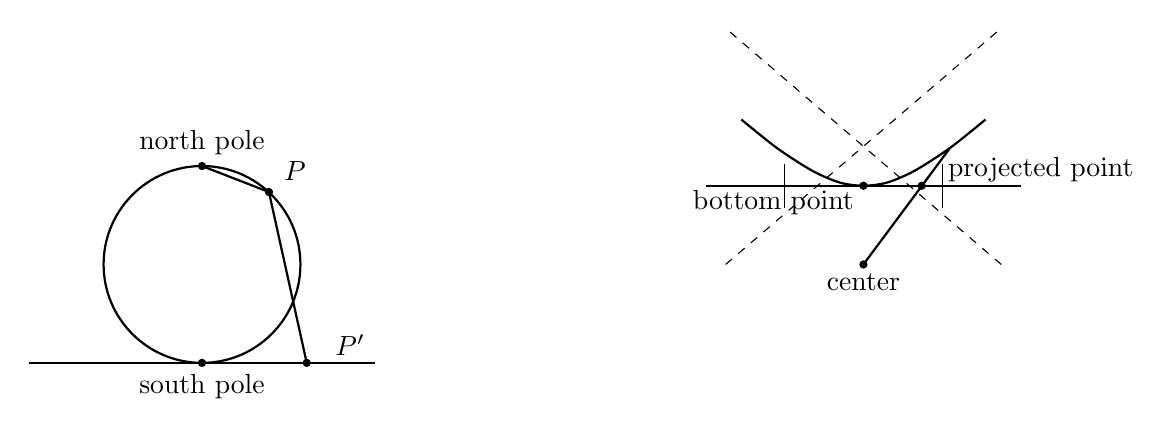
\begin{tikzpicture}[scale=1.0]
\begin{scope}[xshift=-4.2cm]
\draw[thick] (-2.2,-1.25)--(2.2,-1.25);
\draw[thick] (0,0) circle (1.25);
\fill (0,1.25) circle (1.5pt);
\fill (0,-1.25) circle (1.5pt);
\draw (0,1.55) node {north pole};
\draw (0,-1.55) node {south pole};

\fill (0.85,0.92) circle (1.5pt);
\draw (0.92,1.18) node[right] {$P$};
\draw[thick] (0,1.25)--(0.85,0.92)--(1.33,-1.25);
\fill (1.33,-1.25) circle (1.5pt);
\draw (1.57,-1.03) node[right] {$P'$};
\end{scope}

\begin{scope}[xshift=4.2cm]
\draw[thick] (-2.0,1)--(2.0,1);
\draw[dashed] (-1.75,0)--(1.75,3.0);
\draw[dashed] (1.75,0)--(-1.75,3.0);
\draw[thick]
plot[smooth] coordinates
{(-1.55,1.84) (-1.1,1.48) (-0.65,1.19) (-0.3,1.04) (0,1.0) (0.3,1.04) (0.65,1.19) (1.1,1.48) (1.55,1.84)};
\fill (0,0) circle (1.5pt);
\fill (0,1) circle (1.5pt);
\draw (0,-0.22) node {center};
\draw (0,0.78) node[left] {bottom point};
\draw[thick] (0,0)--(1.1,1.48);
\fill (0.74,1.0) circle (1.5pt);
\draw (0.95,1.2) node[right] {projected point};
\draw (-1,0.72) -- (-1,1.28);
\draw (1,0.72) -- (1,1.28);
\end{scope}
\end{tikzpicture}
}%
\caption{左：立体投影は球の北極を無限遠へ写す。右：双曲面は有限な円板へ投影でき、ここでは断面の区間として表されている。座標の歪みは内在的な一様性を損なわない。}
\label{fig:c03-projections}
\end{figure}

\section{負の曲率：平坦空間をはるかに超えて成長する殻}

第三の単連結一様幾何は\(\sin r\)を双曲線正弦に置き換える。その2次元および3次元の単位計量は
\begin{equation}
dh_2^2 = dr^2 + \sinh^2 r\, d\Omega_1^2,
\label{eq:c03-hyperbolic-two}
\end{equation}
\begin{equation}
dh_3^2 = dr^2 + \sinh^2 r\, d\Omega_2^2.
\label{eq:c03-hyperbolic-three}
\end{equation}
座標\(r\)は今や
\begin{equation}
0\le r<\infty.
\end{equation}
の範囲を動く。原点付近では\(\sinh r\approx r\)であるから、この幾何は局所的にユークリッド的である。遠方では、その殻はユークリッド的な殻よりもはるかに速く成長し、決して折り返さない。

成長則は
\begin{equation}
\sin r = \frac{e^{ir}-e^{-ir}}{2i},
\qquad
\sinh r = \frac{e^r-e^{-r}}{2}.
\label{eq:c03-sin-sinh}
\end{equation}
から従う。大きな\(r\)では\(\sinh r\sim e^r/2\)である。したがって2次元では円周は半径とともに指数関数的に成長し、3次元では殻の面積は\(\sinh^2r\sim e^{2r}/4\)として成長する。一様な分布は、遠方の殻上に対応するだけ多くの天体を含む。

大きさ\(d\)の横断的物体に対して、
\begin{equation}
d^2 = \sinh^2 r\, d\theta^2,
\qquad\text{so}\qquad
d\theta = \frac{d}{\sinh r}.
\label{eq:c03-hyperbolic-angle}
\end{equation}
大きな\(r\)では、
\begin{equation}
d\theta \sim 2d\,e^{-r}.
\end{equation}
したがって負の曲率は正の曲率とは逆の兆候を与える。遠方の標準尺は小さすぎるように見え、一方で遠方の殻は平坦空間に比べてあまりに多くの天体を含む。

\begin{classroomqa}
\audiencequestion{動径範囲はどのようにして球面空間と双曲空間を区別するのか。}
\lecturerresponse{単位球面上では、\(r\)は対蹠点\(r=\pi\)で止まる。双曲空間ではそれは際限なく続き、\(0\le r<\infty\)である。殻因子は同じ対照を明らかにする。すなわち\(\sin r\)はゼロに戻るが、\(\sinh r\)は永遠に増大し続ける。\lecturetimestamp{00:52:46--00:53:25}}
\end{classroomqa}

一様性をより不可解でなくする埋め込みが存在する。周囲座標\(T,x,y\)を導入する。ここで\(T\)は単なる埋め込み座標であり、宇宙論的時間では\emph{な}い。そして上側のシート
\begin{equation}
T^2 - x^2 - y^2 = 1.
\label{eq:c03-hyperboloid}
\end{equation}
を取る。周囲空間にローレンツ符号の計量
\begin{equation}
d\ell_{\mathrm{emb}}^2=-dT^2+dx^2+dy^2.
\label{eq:c03-ambient-minkowski}
\end{equation}
を備えさせる。双曲面上に誘導される計量は正定値である。ローレンツ変換は~\eqref{eq:c03-hyperboloid}と~\eqref{eq:c03-ambient-minkowski}の両式を保ち、上側のシートの任意の点を任意の他の点へ移すことができる。その意味で、双曲空間上の原点を変えることは、補助的な周囲空間において時間軸を傾けることに似ている。すべての点は幾何学的に等価である。

双曲面を円板へ投影すると、無限遠の点は境界円に集積する。近傍の領域はほぼ忠実に描かれ、より遠い領域はますます強く圧縮される。これは天使と悪魔の繰り返し図でおなじみのPoincar\'e円板表示である。座標変換は、縁の近くで見かけ上ごく小さい図形を中心へ移し、そこでそれを大きくすることができるが、すべての内在的な長さと角度は保たれる。3次元では対応する模型は円板ではなく球である。\emph{Poincar\'e空間}、\emph{ロバチェフスキー空間}、\emph{一様な負の曲率の空間}という名称は、この同じ局所幾何を指す。

\begin{classroomqa}
\audiencequestion{有限な円板はペンローズ図のようなものか。}
\lecturerresponse{無限の領域が有限な絵の中に表されるという限られた意味では似ている。しかしここでは、円板は時空や因果的無限遠ではなく空間のみを表す。その境界は、図が有限な座標半径に置いているにもかかわらず、内在的な双曲計量において無限に遠い。\lecturetimestamp{01:02:55--01:03:05}}
\end{classroomqa}

\section{曲率半径}

これまでに書いた計量は単位幾何学を記述している。球面や双曲空間に任意の曲率半径を与えるには、すべての長さを定数倍すればよい。板書ではその定数を\(a\)と表すが、後に用いる時間依存の宇宙スケール因子と混同しないよう、ここでは静的な曲率半径を\(R_c\)と呼ぶことにする。計量は長さの二乗を測るので、
\begin{align}
ds_{\mathrm{sph}}^2
  &=R_c^2d\Omega_n^2
   =R_c^2\left(dr^2+\sin^2r\,d\Omega_{n-1}^2\right),\\
ds_{\mathrm{hyp}}^2
  &=R_c^2dh_n^2
   =R_c^2\left(dr^2+\sinh^2r\,d\Omega_{n-1}^2\right).
\label{eq:c03-scaled-curvature}
\end{align}
物理的な動径距離は\(R_cr\)である。\(R_c\)を大きくすると空間の曲がりは小さくなり、一定の断面曲率の大きさは\(1/R_c^2\)としてスケールする。\(R_c\to\infty\)の極限では、二つの曲がった計量はどちらも任意の固定された有限領域上でユークリッド幾何学に近づく。

\begin{classroomqa}
\audiencequestion{球面を二倍の大きさにすると、より曲がるのか、それとも曲がりが小さくなるのか。}
\lecturerresponse{曲がりは小さくなる。授業で最初に示された答えは、バスケットボールと地球を比較することで訂正された。より小さな曲面は、与えられた距離にわたってより急速に曲がる。\(R_c\)を二倍にすると、逆半径の曲率スケールは半分になり、断面曲率\(1/R_c^2\)は四分の一になる。\lecturetimestamp{01:10:14--01:10:56}}
\end{classroomqa}

これにより、3つの幾何学が近傍でなぜ似て見えるかが説明される。\(r\ll1\) では、
\begin{equation}
\sin r=r-\frac{r^3}{6}+\cdots,
\qquad
\sinh r=r+\frac{r^3}{6}+\cdots.
\end{equation}
どちらの曲がった計量でも主要項は平坦な極座標計量であり、曲率は物理的スケール \(L\) にわたって相対次数 \((L/R_c)^2\) の補正として初めて現れる。

\begin{classroomqa}
\audiencequestion{観測は、空間が平坦か、球面か、双曲かどうかを教えてくれるだろうか。}
\lecturerresponse{観測は、観測可能な領域が平坦に非常に近いことを教えてくれる。教室での粗い見積もりでは、曲率効果に対する1パーセントの上限は、\((L/R_c)^2\lesssim10^{-2}\) であるため、\(R_c\) が可視領域の大きさの少なくとも約10倍であることを意味していた。対応する曲率体積は、すると少なくともおよそ \(10^3\) の可視体積となる。これは講義での桁の見積もりであり、現在の精密データの引用ではなく、厳密な平坦性は依然として \(R_c=\infty\) の可能性である。\lecturetimestamp{01:11:00--01:13:37}}
\end{classroomqa}

\section{平坦だが有限：トーラス}

ここで、平坦、球面、双曲空間が唯一の一様な可能性であるという記述を訂正しなければならない。それらは3つの単連結な定曲率幾何学である。平坦な空間は非自明な大域トポロジーを持つこともできる。

ユークリッド長方形から始める。その左辺を点ごとに右辺と同一視し、底辺を上辺と同一視する。どの辺を横切っても反対側の辺を通って戻る。局所計量は \(dx^2+dy^2\) のままだが、大域空間は周期的で有限である。この商は平坦な2次元トーラス \(T^2\) である。1つの周期的次元は円 \(T^1\) を与え、直方体の向かい合う面を同一視すると平坦な3次元トーラス \(T^3\) が得られ、この構成は任意の次元数に拡張される。

\begin{figure}[htbp]
\centering
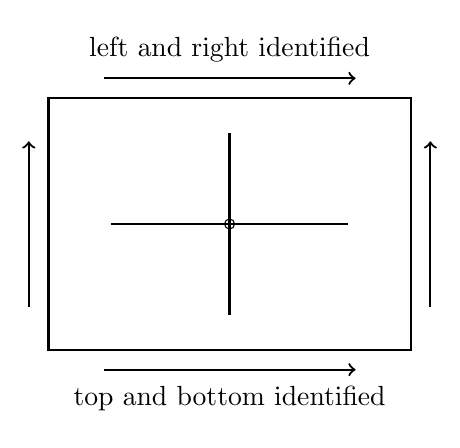
\begin{tikzpicture}[scale=1.0]
\draw[thick] (0,0) rectangle (4.6,3.2);

\draw[->,thick] (0.7,3.45)--(3.9,3.45);
\draw[->,thick] (0.7,-0.25)--(3.9,-0.25);

\draw[->,thick] (-0.25,0.55)--(-0.25,2.65);
\draw[->,thick] (4.85,0.55)--(4.85,2.65);

\draw[thick] (0.8,1.6)--(3.8,1.6);
\draw[thick] (2.3,0.45)--(2.3,2.75);

\draw (2.3,1.6) circle (1.8pt);

\draw (2.3,-0.62) node {top and bottom identified};
\draw (2.3,3.82) node {left and right identified};
\end{tikzpicture}
\caption{長方形の向かい合う辺を同一視して構成した平坦なトーラス。辺は境界ではなく、対にされた点は商空間の同じ点である。}
\label{fig:c03-flat-torus}
\end{figure}

\begin{classroomqa}
\audiencequestion{したがって宇宙は平坦かつ有限でありうるか。}
\lecturerresponse{はい。平坦性は計量についての局所的な言明であり、有限性はトポロジーについての大域的な言明でありうる。十分に大きな3次元トーラスは、全体積が有限であっても、我々が観測できる領域全体でユークリッド的に見えるだろう。\lecturetimestamp{01:13:37--01:17:59}}
\end{classroomqa}

普遍被覆の描像は観測上の帰結を明瞭にする。辺を同一視する代わりに、無限のユークリッド平面を基本長方形のコピーで敷き詰める。トーラス内の1つの物体はすべてのコピーに1回ずつ現れる。3次元では、コピーは周期的な結晶のような配列をなす。

\begin{classroomqa}
\audiencequestion{我々は気づかずにトーラス状の宇宙に住むことができるだろうか。}
\lecturerresponse{はい、基本セルが光が我々に到達した領域より大きければ可能である。もし十分に小さければ、光は同一視を横断でき、我々は同じ銀河の繰り返し像を、おそらくは我々自身の近傍の繰り返しの眺めさえも、異なる方向に見るだろう。どちらの場合でも局所幾何学は平坦のままだろう。\lecturetimestamp{01:18:16--01:22:04}}
\end{classroomqa}

\begin{classroomqa}
\audiencequestion{なぜ球面はその対蹠点で止まるのに、トーラスは繰り返すのか。}
\lecturerresponse{球面では、周囲の殻は \(r=\pi\) で真にゼロに縮む。すべての動径方向は対蹠点で出会う。トーラスでは、選んだ長方形セルの縁は決して縮まない。それは同じ大きさの向かい合う縁と同一視されるので、それを横切ることは周期的な座標記述で同じ空間を続けることになる。\lecturetimestamp{01:22:06--01:23:02}}
\end{classroomqa}

\section{空間から時空へ}

ここで時間を復活させることができる。光速 \(c=1\) とする単位では、ミンコフスキー計量は
\begin{equation}
ds^2 = -dt^2 + dx^2 + dy^2 + dz^2.
\label{eq:c03-minkowski}
\end{equation}
符号の規約は選択である。重要なのは、時間項が空間項と反対の符号を持つことである。光線はヌル軌道に従い、
\begin{equation}
ds^2 = 0.
\end{equation}
\(x\) に沿った運動のみでは、
\begin{equation}
-dt^2 + dx^2 = 0
\qquad\Rightarrow\qquad
dx = \pm dt.
\label{eq:c03-null-flat}
\end{equation}
2つの符号は、光が単位速さで左または右に進むことを表す。

宇宙論では、固有時間項 \(-dt^2\) を保ち、ユークリッド空間部分を一様な空間計量に置き換え、その全体的なスケールを時間とともに変化させる。このスケール因子を \(a(t)\) と表す。これはもはや、静的比較で用いた固定された半径 \(R_c\) ではなく、動的な関数である。

描像可能な\(2+1\)次元の例として、
\begin{equation}
ds^2 = -dt^2 + a(t)^2 d\Omega_2^2.
\label{eq:c03-two-plus-one}
\end{equation}
を取る。各固定された\(t\)において、空間は半径\(a(t)\)の\(2\)球面である。これらの球面を時間方向に積み重ねると時空が得られる。よく知られた\(3+1\)次元の構成は
\begin{equation}
ds^2 = -dt^2 + a(t)^2 d\Sigma^2,
\label{eq:c03-frw-general}
\end{equation}
であり、ここで\(d\Sigma^2\)は時間に依存しない単位空間計量である。単連結な三つの場合は
\begin{align}
\text{flat:}\quad
ds^2&=-dt^2+a(t)^2\left(dx^2+dy^2+dz^2\right),\label{eq:c03-frw-flat}\\
\text{spherical:}\quad
ds^2&=-dt^2+a(t)^2d\Omega_3^2,\label{eq:c03-frw-spherical}\\
\text{hyperbolic:}\quad
ds^2&=-dt^2+a(t)^2dh_3^2.\label{eq:c03-frw-hyperbolic}
\end{align}
である。\(a(t)\)が変化する間、共動座標の相対的なスケールは固定されている。球面および双曲型の規格化では、\(a(t)\)は瞬間的な曲率半径でもある。平坦な場合、その絶対規格化は共動座標に吸収できる。

ハッブル則は、いかなる重力場の方程式も課される前に導かれる。固定された座標間隔\(\chi\)を持つ近傍の二つの共動点を考える。それらの物理的間隔は
\begin{equation}
D(t)=a(t)\chi.
\label{eq:c03-comoving-distance}
\end{equation}
である。\(\chi\)を固定して微分すると
\begin{equation}
V=\dot D=\dot a(t)\chi.
\end{equation}
が得られる。\(\chi\)を消去すると、
\begin{equation}
V = \frac{\dot a}{a} D.
\label{eq:c03-hubble-law}
\end{equation}
したがって
\begin{equation}
H = \frac{\dot a}{a}.
\label{eq:c03-hubble-parameter}
\end{equation}
である。これは一様な膨張または収縮に対する運動学的な恒等式である。これは三つの空間幾何すべてに当てはまる：\(\dot a>0\)は後退を与え、\(\dot a<0\)は接近を与える。

幾何学だけでは\(a(t)\)を決定しない。
\begin{equation}
a(t)\propto t^{2/3},
\qquad
a(t)\propto t^{1/2},
\qquad
a(t)\propto e^{Ht}
\end{equation}
のような関数はすべて一様計量の仮定に適合するが、異なる宇宙の物質およびエネルギー内容を記述する。一般相対性理論が、それらの中から選び出す力学方程式を与える。得られるフリードマン方程式はまた、平坦・球面・双曲型の場合を、先に展開したニュートン宇宙論のゼロ・負・正エネルギーの選択肢と結びつけるであろう。

\begin{classroomqa}
\audiencequestion{幾何学と宇宙の進化は、これらのモデルよりもはるかに複雑であり得るだろうか？}
\lecturerresponse{もちろんである。一様性と等方性は制限的な仮定であり、それらが自然で、大スケールで観測的に成功しており、数学的に扱いやすいために選ばれている。はるかに複雑な幾何学と進化が存在する。重要な力学上の問題は、初期に不規則なモデルの広いクラスがこれらの単純な一様形の一つへと進化するかどうかである。\lecturetimestamp{01:36:00--01:36:50}}
\end{classroomqa}

\begin{classroomqa}
\audiencequestion{\(3\)球面は四次元物体の境界だろうか？}
\lecturerresponse{埋め込みとしてそのように表すことはできるが、宇宙論的空間は\(3\)球面そのものである。それは三つの内在的次元を持ち、境界を持たない。四次元ユークリッド的描像は任意の足場であり、式~\eqref{eq:c03-three-sphere}がすでに幾何学を完全に定義している。\lecturetimestamp{01:36:55--01:37:59}}
\end{classroomqa}

\begin{classroomqa}
\audiencequestion{曲率テストに必要な距離を得る唯一の方法は光度だろうか？}
\lecturerresponse{いいえ。スペクトル線は赤方偏移を同定し、近傍の距離はしごはハッブル関係を較正し、超新星はほぼ標準的な光度を与える。これらの方法は孤立して信頼されるのではなく、相互に検証される。逆二乗光度則でさえ、光の波面の面積が\(r^2\)、\(\sin^2r\)、または\(\sinh^2r\)によって定まるため、幾何学に依存する。いくつかの観測量の一致が、ほぼ平坦であることを支持するのである。\lecturetimestamp{01:38:00--01:41:07}}
\end{classroomqa}

\section{引き継ぐべきこと}

一様宇宙の幾何学は、任意の観測者の周りの殻の成長から読み取ることができる：
\begin{equation}
f(r)=
\begin{cases}
r, & \text{flat space},\\
\sin r, & \text{positive curvature},\\
\sinh r, & \text{negative curvature}.
\end{cases}
\end{equation}
空間計量は\(dr^2+f(r)^2d\Omega_{n-1}^2\)である。同じ関数が角度サイズと殻上で利用可能な天体の数を制御するので、曲率は直接的な観測的意味を持つ。大きな曲率半径はこれらの違いを局所的に隠し、トーラス的同一視は、局所曲率だけでは大域的サイズやトポロジーを決定しないことを示す。

\(-dt^2\)と共通因子\(a(t)^2\)を加えると、三つの一様空間計量のいずれもが宇宙論的時空になる。それは直ちに\(H=\dot a/a\)を伴う\(V=HD\)を与えるが、\(a(t)\)を未決定のまま残す。したがって次の段階は、幾何学の別の練習ではない。それは力学の問題である：アインシュタイン方程式を用いて、物質、放射、曲率、その他のエネルギー形態がどのようにスケール因子を進化させるかを決定するのである。
